\documentclass[10pt,a4paper]{article}
\usepackage{fullpage}
\usepackage{amsfonts, amsmath, pifont}
\usepackage{amsthm}
\usepackage{graphicx}
\usepackage{subfig}
\usepackage{float}
\usepackage{longtable}
\usepackage{tkz-euclide}
\usepackage{titling}
\usepackage{booktabs}
\usepackage{hyperref}
\usepackage{comment}
\usepackage{tikz}
\usepackage{pgfplots}
\pgfplotsset{compat=1.13}

\setlength{\droptitle}{-7em} 
\title{CENG519 - Phase 2 Report}
\author{
  Cansu Eskici\\
  2588036}
\begin{document}
\maketitle
\section*{Introduction}
My choice of covert channel was \textit{Using options fields in TCP headers (such as timestamps) for data hiding.} 
For this purpose, I choose timestamps from TCP header options. 
This value can be used to synchronize clocks between the sender and receiver, or it can be used to measure the round-trip time of packets.
For my research, I used the following resources:
\begin{itemize}
    \item \href{https://web.mit.edu/greenie/Public/petspaper.pdf}{Covert Messaging through TCP Timestamps}
    \item \href{https://scapy.readthedocs.io/en/latest/}{Scapy Documentation}
\end{itemize}

First one is an academic paper that proposes a detailed and well structured algorithm for utilizing TCP timestamps for covert messaging. In my implementation, I did not use the same algorithm design, however it was very helpful to understand the concept of covert messaging through TCP timestamps.

The second one is Scapy documentation, I used Scapy to implement the communication between TCP client and server. 

\section*{Development}

For this project, I created a covert communication channel utilizing TCP timestamps to encode and decode messages.

The sender encodes a given message into binary bits, splits it into chunks of a specified size (bits), and calculates a value for each chunk based on its binary representation.
To create the illusion of the monotonically increasing timestamps, timestamp\_value is incremented by the calculated value for each chunk.
These timestamps are embedded in TCP packets and sent to a specified destination (dst\_ip and dst\_port). 

The receiver captures these packets, extracts the timestamps, and reconstructs the original message by calculating the subtracting the previous timestamp\_value from the current one, and decoding the binary representation of the message.
Lastly, receiver also handles a termination signal (timestamp\_value = 0) to indicate the end of the transmission. The receiver reconstructs the original message upon receiving the termination signal.


\section*{Experiments}
For experimentation, the independent variables were 
\begin{itemize}
    \item \textit{Bits}, used for encoding each chunk of the message was varied across four values: 7, 8, 16, and 25.
    \item \textit{Delay}, was tested with three values: 0.01 seconds, 0.10 seconds, and 0.15 seconds.
    \item \textit{Message}, Different messages of varying lengths and content were used to test the channel's performance. The messages varied across 21, 75, 141 and 299 bytes.

\end{itemize}

The dependent variables were the average elapsed time, the capacity of the covert channel with its \%95 confidence intervals.
In order to make sure that the decoded message is correct, original message was compared with the decoded message in each experiment. 


\section*{Results}

\begin{figure}[H]
\centering
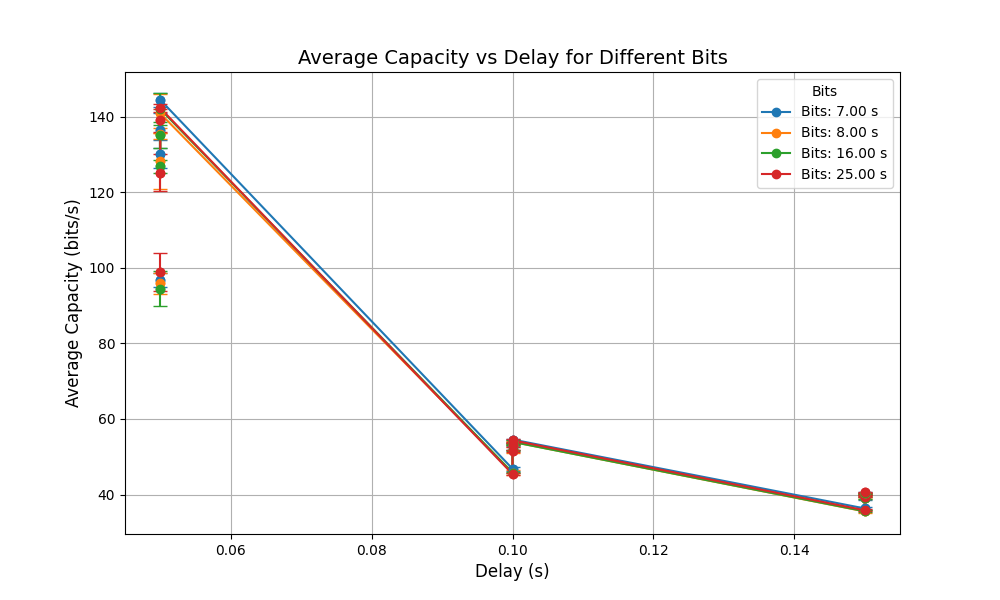
\includegraphics[width=0.87\textwidth]{ave_cap_vs_delay.png}
\caption{Average Capacity vs Delay}

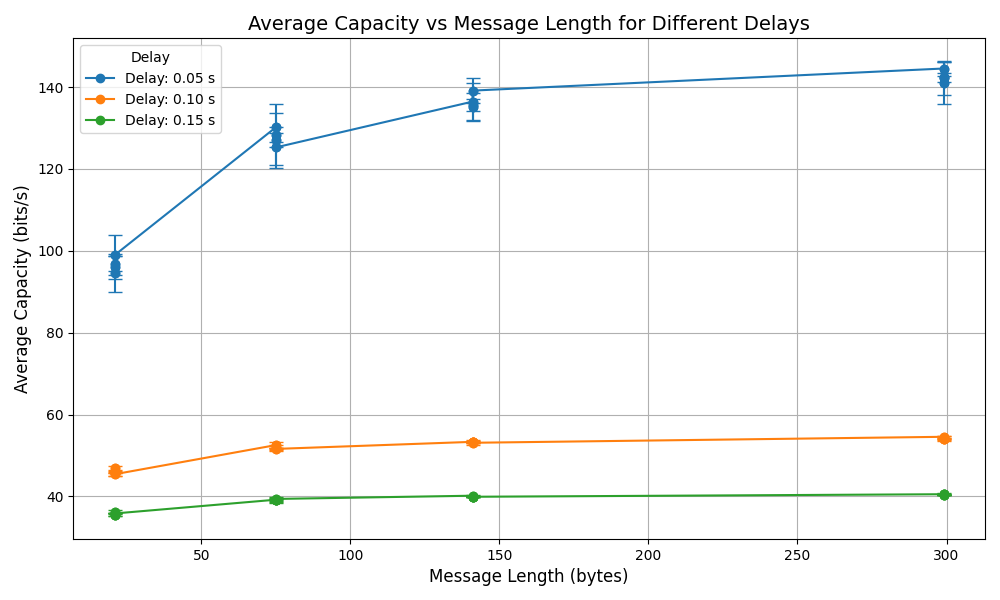
\includegraphics[width=0.78\textwidth]{ave_cap_vs_len.png}
\caption{Average Capacity vs Number of Bits}
\end{figure}

By looking at the figures above, one can see that the average capacity of the covert channel is affected by the delay and the number of bits used for encoding.
The average capacity of the covert channel decreases as the delay increases. This is because a longer delay means that the sender has to wait longer before sending the next packet, which reduces the overall throughput of the channel.
Similarly, the average capacity of the covert channel decreases as the number of bits used for encoding increases. This is because a larger number of bits means that more time is needed to encode and decode the message, which reduces the overall throughput of the channel.
In addition, the average elapsed time was also recorded for each experiment. Consistent with the findings, the elapsed time was long when the capacity of the covert channel was low, and vice versa. Also, no corrupt messages were received during the experiments, proving the reliability of the covert channel. The complete results of the experimentation can be found the table in the next page.

\begin{table}[H]
    \centering
    \begin{tabular}{|c|c|c|c|c|c|}
    \hline
    \textbf{Bits} & \textbf{Delay (s)} & \textbf{Length (bytes)} & \textbf{Elapsed Time (s)} & \textbf{Avg Cap (bits/s)} & \textbf{Conf Interval} \\ \hline
    7 & 0.05 & 21 & 1.7355 & 96.82 & [95.00, 98.63] \\ \hline
    7 & 0.10 & 21 & 3.5885 & 46.82 & [46.32, 47.31] \\ \hline
    7 & 0.15 & 21 & 4.6281 & 36.30 & [36.00, 36.60] \\ \hline
    7 & 0.05 & 75 & 4.6115 & 130.16 & [126.54, 133.77] \\ \hline
    7 & 0.10 & 75 & 11.4225 & 52.53 & [51.88, 53.18] \\ \hline
    7 & 0.15 & 75 & 15.3137 & 39.19 & [38.48, 39.89] \\ \hline
    7 & 0.05 & 141 & 8.2705 & 136.45 & [131.91, 141.00] \\ \hline
    7 & 0.10 & 141 & 21.1530 & 53.33 & [52.97, 53.68] \\ \hline
    7 & 0.15 & 141 & 28.0808 & 40.17 & [40.05, 40.29] \\ \hline
    7 & 0.05 & 299 & 16.5499 & 144.54 & [142.74, 146.35] \\ \hline
    7 & 0.10 & 299 & 43.8405 & 54.56 & [54.37, 54.75] \\ \hline
    7 & 0.15 & 299 & 59.0114 & 40.53 & [40.40, 40.67] \\ \hline
    8 & 0.05 & 21 & 1.7519 & 95.93 & [93.11, 98.76] \\ \hline
    8 & 0.10 & 21 & 3.6691 & 45.79 & [45.06, 46.53] \\ \hline
    8 & 0.15 & 21 & 4.7316 & 35.51 & [35.10, 35.92] \\ \hline
    8 & 0.05 & 75 & 4.6798 & 128.40 & [120.94, 135.86] \\ \hline
    8 & 0.10 & 75 & 11.5742 & 51.84 & [51.11, 52.57] \\ \hline
    8 & 0.15 & 75 & 15.3337 & 39.13 & [38.92, 39.34] \\ \hline
    8 & 0.05 & 141 & 8.3222 & 135.55 & [134.11, 136.98] \\ \hline
    8 & 0.10 & 141 & 21.1872 & 53.24 & [53.06, 53.42] \\ \hline
    8 & 0.15 & 141 & 28.2895 & 39.87 & [39.78, 39.96] \\ \hline
    8 & 0.05 & 299 & 16.9810 & 140.95 & [135.76, 146.13] \\ \hline
    8 & 0.10 & 299 & 44.3362 & 53.95 & [53.78, 54.13] \\ \hline
    8 & 0.15 & 299 & 59.3114 & 40.33 & [40.25, 40.41] \\ \hline
    16 & 0.05 & 21 & 1.7790 & 94.53 & [89.90, 99.16] \\ \hline
    16 & 0.10 & 21 & 3.6703 & 45.77 & [45.66, 45.88] \\ \hline
    16 & 0.15 & 21 & 4.7239 & 35.56 & [35.26, 35.87] \\ \hline
    16 & 0.05 & 75 & 4.7256 & 126.98 & [125.27, 128.68] \\ \hline
    16 & 0.10 & 75 & 11.6033 & 51.71 & [51.60, 51.82] \\ \hline
    16 & 0.15 & 75 & 15.3463 & 39.10 & [38.75, 39.45] \\ \hline
    16 & 0.05 & 141 & 8.3474 & 135.17 & [131.70, 138.64] \\ \hline
    16 & 0.10 & 141 & 21.1819 & 53.25 & [53.11, 53.39] \\ \hline
    16 & 0.15 & 141 & 28.3008 & 39.86 & [39.74, 39.97] \\ \hline
    16 & 0.05 & 299 & 16.8394 & 142.10 & [137.98, 146.22] \\ \hline
    16 & 0.10 & 299 & 44.3444 & 53.94 & [53.57, 54.32] \\ \hline
    16 & 0.15 & 299 & 59.3330 & 40.31 & [40.25, 40.38] \\ \hline
    25 & 0.05 & 21 & 1.6994 & 98.97 & [94.00, 103.93] \\ \hline
    25 & 0.10 & 21 & 3.6991 & 45.42 & [45.07, 45.77] \\ \hline
    25 & 0.15 & 21 & 4.6888 & 35.83 & [35.62, 36.05] \\ \hline
    25 & 0.05 & 75 & 4.7933 & 125.26 & [120.28, 130.24] \\ \hline
    25 & 0.10 & 75 & 11.6269 & 51.60 & [51.35, 51.86] \\ \hline
    25 & 0.15 & 75 & 15.2357 & 39.38 & [39.23, 39.53] \\ \hline
    25 & 0.05 & 141 & 8.1086 & 139.14 & [136.08, 142.21] \\ \hline
    25 & 0.10 & 141 & 21.2442 & 53.10 & [52.58, 53.62] \\ \hline
    25 & 0.15 & 141 & 28.2664 & 39.91 & [39.81, 40.00] \\ \hline
    25 & 0.05 & 299 & 16.8003 & 142.38 & [141.33, 143.43] \\ \hline
    25 & 0.10 & 299 & 44.0127 & 54.35 & [53.92, 54.78] \\ \hline
    25 & 0.15 & 299 & 58.8517 & 40.64 & [40.50, 40.79] \\ \hline
    \end{tabular}
    \caption{Average Elapsed Time, Capacity, and Confidence Intervals for Different Configurations}
    \label{tab:results}
\end{table}




\end{document}

